\chapter{Networks}
\label{chap:network}

Although there are many kinds of computer networks created, the vast majority of network equipment is based on the TCP/IP stack, which we will cover in these notes. These course notes focus on explaining how the network is implemented and the properties that arise from the implementation. Some reference material for network programming is included at the end of the chapter, but the exercises are intended as the main way to learn this.

\section{OSI layers}
The OSI layers are a model that explains the implementation of the internet. Each of the layers in the OSI model relies on the previous layer and makes certain assumptions about it. Using the services provided by the underlying layer, each layer can add new services. There are several different versions of the OSI model, with differing numbers of layers and various names for those layers. For this course we will only consider the commonly used 5 layer model shown below. Just make sure to remember that different representations do exist.

\begin{figure}
  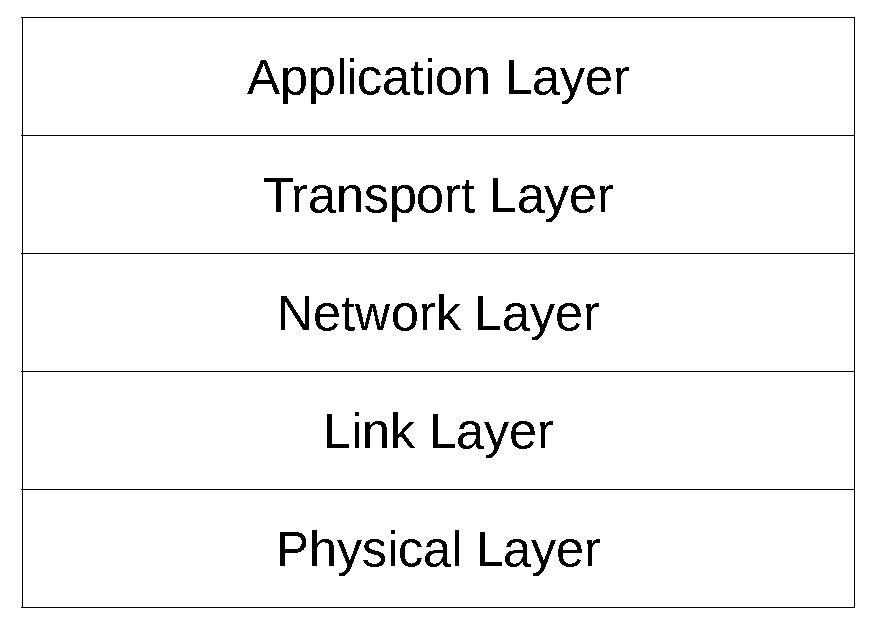
\includegraphics[width=0.5\textwidth]{img/osi.pdf}
  \centering
  \caption{The 5 layer OSI model}
  \label{fig:osi}
\end{figure}

By using a layered model we can seperate out functionality, to aid modelling, but also product design and deployment. By letting individual components (software or hardware) only need to meet the requirements of an individual layer, then companies or developers can more easilly create small components that can be of use to the wider network. This has greatly aided the very fast deployment of a global network of devices, which would not be possible if each user needed to implement an entire end to end system. The OSI model is intended to describe many kinds of networks, but in the text here we map the concepts to the implementation on global internet and consider this the only implementation. 

\section{Physical layer}
The physical layer is the lowest layer in the OSI model and is concerned with transmission of bits via various propagation media. The first networks were implemented as wired networks, propagating electrical signals through a shared copper wire. Modern implementations use radio signals, to implement services such as Wi-Fi and 3/4/5G. 

The physical layer provides the service of sending and receiving bits. It is important to note that due to properties of the propagation medium, the timings, bandwidth, and error correction properties are different. Each of the layers above needs to accept this, such that the layers work similarly with different physical layers.

\subsection{Sharing a medium}
The most significant work done by the physical layer is the ability to transmit messages on a shared medium, without any out-of-band control mechanism. The primary method for solving this is the use of a multiple-access protocol. For both (wired) Ethernet and Wi-Fi, the protocol is the carrier-sense multiple-access collision, CSMA, protocol. The protocol requires that each host can "sense" if data is being sent, and refrains from sending data which would cause a collision, making the data impossible to read. Since there is no out-of-band communication, collisions will eventually happen when two hosts communicate. The CSMA protocol uses a concept of exponential back-off with random starting values to ensure that collisions are eventually resolved.

\subsection{Sharing with radio signals}
For radio-based networks, it is possible to have a situation where the base station (the Wi-Fi access point) is placed between two hosts, such that neither can sense the other host's signals. In this case the CSMA protocol is extended to use collision avoidance, as the detection is not always possible. The concept is explored in this animated video: \url{https://www.youtube.com/watch?v=iKn0GzF5-IU}.

\subsection{Connecting: Hub}
Since the physical layer is about transmitting signals, and a shared media is supported, the physical layer allows multiple machines to be joined. For Ethernet (wired) networks, a hub can be used to physically connect multiple devices. With a network connected by a hub, the entire bandwidth for the network is shared with all hosts, resulting in poor scalability. If a network comprises 100 hosts and is using 100 Mbps Ethernet, each host will reach less than 1 Mbps if all hosts attempt to communicate at full speed.

\section{Link layer}

With a physical layer that is capable of transmitting bits, the link layer provides the option for addressing a single host. The bits are \emph{framed} to allow sending a number of bits. Since the physical layer is expected to be using a shared medium, the link layer assumes that all frames are broadcast to every host.

\subsection{Addressing network cards: MAC}
To solve the problem of sending a frame to a particular host, the link layer adds \emph{media access control}, MAC, addresses. Every network device has a globally unique address that is typically burned into the device but can be changed in some cases. When a host wishes to communicate with another host, a frame is transmitted on the physical medium, containing the MAC address of the recipient and sender.

The format of the MAC address is using six dual-digit hexadecimal numbers, for instance: \texttt{01:23:45:67:89:ab}. The special address \texttt{ff:ff:ff:ff:ff:ff} is used for broadcasting frames to all recipients.

\subsection{Connecting: Switch}
To make larger networks more efficient, a switch can be used in place of a hub. Where the hub operates on the physical layer, a switch operates on the link layer and forwards frames. When a switch is powered on, it has no knowledge of the network. Each frame it receives, it will broadcast to all other ports with a cable plugged in. For each package it receives, it will record the sender MAC address as well as the originating port. Since each MAC address is globally unique, the switch can use this simple scheme to learn where to send a frame and can avoid broadcasting to the entire network. Note that this feature works without any configuration, and even supports networks of networks, as the switch will allow mapping multiple MAC addresses to a single port. If a host is moved to another port, there will be a short period where the switch will forward frames incorrectly, until it sees a package from the new port.

\subsection{Switches can increase available bandwidth}
Once the network has levels, or just a large number of hosts, switches become a crucial component in ensuring performance of the network. More expensive switches can allow multiple parallel full-duplex data paths, such that multiple pairs of ports may use the full bandwidth. This allows the network to scale better with the addition of multiple hosts but may still have bottlenecks if there is cross-switch communication.

\subsection{Transmission errors}
Since the physical layer \emph{may} have transmission errors, the link frames typically include a simple checksum that the receiver verifies. If the checksum is incorrect, or any parts of the frame are invalid, the frame is \emph{dropped} with no notification to the sender.

\section{Network layer}
With a layer that supports sending frames, the network layer adds routing and global addressing. While we \emph{can} build larger networks with a switch, the idea of broadcasting becomes problematic for a global network. 

\subsection{Addressing hosts: IP address}
Because the MAC address is fixed, it is not usable for global routing. Imagine that a core router on the internet would need to keep a list of all MAC addresses for all machines in Europe. The size and maintenance of such a list would be an almost impossible task.

To simplify routing, each host on the network layer has at least one IP address, used to transmit \emph{packages}. The IP addresses are assigned in a hierarchical manner, such that a geographic region has a large range, which is then divided into smaller and smaller ranges. At the bottom is the internet service provider, ISP, who owns one or more ranges. From these ranges they assign one or more IP addresses to their customers.

The hierarchy is important when considering global-scale routing. Instead of having a core router that keeps track of all IPs for Europe, it can just know that one of the ports "eventually leads to Europe" and then assign a few IP ranges to that port.

\subsection{IP, CIDR, networks and masks}
The IP addresses are 32 bit numbers, and usually presented as four 8-bit decimal numbers, called the dotted-decimal notation: \texttt{123.211.8.111}. The routing works locally by comparing one IP address with another, using bitwise \texttt{XOR}. By \texttt{XOR}'ing two IP addresses, any bits that are the same will be zero. The subnet mask then defines what bits are ignored, so we can use bitwise \texttt{AND} on the result. After these two operations, the result will only be all zero bits if two IP addresses are on the same subnet.

As an example, consider the two IP addresses \texttt{192.168.0.8} and \texttt{192.168.0.37}. Given a subnet mask of \texttt{255.255.255.192}, we can apply the \texttt{XOR} operation to the two numbers and get \texttt{0.0.0.45}. When we apply the \texttt{AND} operation to the result we get \texttt{0.0.0.0}, meaning that the two hosts are on the same subnet.

As the subnet masks are always constructed with leading zeroes (i.e. it is not valid to use \texttt{255.0.255.0}), we can simply count the number of leading bits in the mask. This gives the classless interdomain routing notation, where we supply the IP address and number of bits in a compact notation: \texttt{192.168.0.0/26}. This notation is equivalent to supplying an IP address and a subnet mask, as we can convert trivially between the two.

\subsection{Packets}
So far we have mentioned packages a few times without really describing what they are. Most messages sent over the network are small (maybe only a couple of hundred bytes in length), but there are manay messages that considerably larger than this. If a file of several GB in size was sent continuously over the network it would take considerable amount of time, and no other communication could take place in that time. This is how traditional network communication such as old landline phones used to opperate and is has the additional inefficency of the space for the message on the network needs to be reserved, even if no message is actually being sent at that time. Modern networks split up messages into packets, typically of no more than 1500B in size. These packets can be interleaved with other messages being sent over the network to share the available resources. Packets may be recieved out of order at the recieving end of the communication, in which case the protocols discussed below will re-order them correctly before passing the message on to the application layer.

\subsection{Connecting networks: Router}
If we consider a package sent from a home-user in Europe to a server in the USA, the package will initially be sent to the \emph{uplink} port of the routers, until it reaches a router that can cross the Atlantic ocean. After it has crossed the Atlantic ocean, it will reach more and more specific IP ranges until it arrives at the destination. This system allows each router to know only general directions, simplified as "one port for away, multiple closer". As mentioned in the video, routing is often done with "longest prefix matching", where multiple rules are stored as a tuple of: \texttt{(destination port, IP pattern in CIDR)}. The router can then sort the rules by the number of fixed bits (i.e. the \texttt{/x} part of the CIDR address), and use the first forwarding rule where the bits match. This approach allows the router to store broad "general rules" and then selectively change smaller ranges. As the only operations required are \texttt{XOR} + \texttt{AND}, it can be performed efficiently in hardware.

\subsection{A router is a host}
The router device itself works on the network layer, such that it can read the IP address. It can be considered a specialized computer, because the first routers were simply ordinary computers with multiple network cards. Unlike the switch and hub, a router is visible on the network and is addressable with its own IP addresses.

To function correctly, a router needs to know what ranges its ports are connected to, which requires manual configuration. As the network can also change, due to links being created and removed, as well as traffic changes and fluctuating transfer costs, the routers need to be dynamically updated.

\subsection{Updating routing tables}
The dynamic updates are handled inside each owners’ network, and across the networks using various protocols, constantly measuring capabilities, traffic load, and costs. One of the protocols for communicating routes between network owners is called the Border Gateway Protocol and is unfortunately not secure yet. Bad actors can incorrectly advertise short and routes, which causes the networks to start sending all traffic over a particular link, either for disruption or eavesdropping purposes. Occasionally this also happens due to human errors, leaving parts of the internet unreachable for periods of time.

For an overview of the layers until now, and the different components that connect them, there is an animated video here: \url{https://www.youtube.com/watch?v=1z0ULvg_pW8}.

\subsection{Packet loss}
Each point on the network, be it routers or hosts, will maintain some cache for the storing of packets. The recieving of packets, writing them to cache, waiting for them to be transmitted, and the time taken to write them onto the network all conmtibute to a nodal delay, e.g. the delay in sending a packet at a given node. Nodes will have a finite sending speed and if packets are recieved faster than they can be sent then the local cache will fill up. If this state persists then eventually the cache will fill and packet loss will occur, where a packet is discarded or overwritten. Any information in this packet will be permanently lost. 

\section{Transport layer}
With a network layer that is capable of transmitting a package from one host to another, the transport layer provides one protocol for doing just that: User Datagram Protocol, UDP.

\subsection{Adding ports}
A datagram in UDP adds only a single feature to the service provided by the network layer: ports. To allow multiple processes on a given host to use the network, UDP adds a 16-bit port number. When describing and address on the transport layer, the port number is often added to the IP address or hostname after a colon: \texttt{192.168.0.1:456}. The operating system kernel will use the IP address and port number to deliver packages to a particular process (More on this below). However, since UDP uses the network layer, there is no acknowledgement of receipt and no signals if a package is lost. Because the routers update dynamically, it is also possible for packages to reach the destination via different routes, causing packages to arrive in a different order than they were sent.

UDP does not make any attempt to detect packet loss, and so it is up to an Application to determine when to resend data or not. Despite this, UDP can be acceptable for some cases such as game updates or video streams, where we would rather loose a frame than have a stuttering video. But for many other cases, such as transferring a file or dataset, the UDP service is not useful.

Note that port numbers can be anything up to ~65000, but that it is common practice to avoid 0-2000ish as these are reserved for 'well-known' services. For example, most websites are hosted on port 80, and to keep functionality clear we politely avoid using 80 for non-website applications.

\subsection{Transmission control protocol: TCP}
The Transmission Control Protocol, TCP, is the most widely used protocol and most often used with IP to form TCP/IP. The TCP protocol builds a reliable transfer stream on top of an unreliable delivery provided by the network layer. The protocol itself is very robust, with understandable mechanics, but can require some trials to accept that it works in all cases.

\subsection{Establishing a connection}
Since the network layer does not tell us if a package has been delivered, the TCP protocol uses \emph{acknowledgements}, ACKs, to report receipt of a package. Before a connection is establish, the client sends a special SYN message, and awaits an ACK, and sends an ACK. This exchange happens before any actual data is transmitted but allows for "piggy backing" data on the last ACK message. When designing an application, it is important to know that this adds an overhead for each established connection, and thus connections should preferably be reused where possible. 

\subsection{A simple stop-and-go TCP-like protocol}
Once the connection is established, data can flow, but due to the network layers unreliability, we can receive packages out-of-order or lose them. For a simple protocol, we can just drop out-of-order packages, treating them as lost. The remaining problem has two cases: loss of package and loss of ACK. Since the sender cannot know which of these has occurred, it assumes the data is lost, and re-transmits it after a timeout has occurred while waiting for an ACK. If we prematurely hit a timeout, we will re-send a received package, but this is the same case as a lost ACK will produce.

The recipient can simply discard a package it has already received, so if we add a package number, called a sequence number\footnote{In the text and the video, we use a number pr. package. In the real TCP protocol, the sequence number counts bytes to support split packages.}, to the package, it is trivial for the recipient to know which packages are new and which are retransmits. It should be fairly simple to convince oneself that this works in all cases, in the sense that the recipient will eventually get the package, and the sender will eventually get an ACK.

\subsection{Improving bandwidth with latency hiding}
However, due to the communication delay, we are waiting some of the time, instead of communicating. For even moderate communication delays, this results in poor utilization. To work around this, the TCP protocol allows multiple packages to be "in-flight", so the communication can occur with full bandwidth. This requires that the sender needs to keep track of which packages have gotten an ACK and which are still pending. We also need to keep copies of multiple packages, such that we can retransmit them if required. This does not change the way the simple stop-n-go protocol works, it simply adds a counter on the sender side. The choice of "how many" is done with a ramp-up process, increasing until no improvements are seen, which further adds to the delay of new connections.

\subsection{Minimizing retransmission}
We could stop there, and be happy that it works, but if we get packages out-of-order it means not being able to send the ACK, and many in-flight packages needs to be retransmitted. This is solved in TCP by keeping a receive buffer, allowing packages to arrive in out-of-order. This does not change the protocol, except that the recipient needs to send an ACK, only when there are no "holes" in the sequence of received packages. This is simplified a bit in TCP, where an ACK is interpreted as vouching for all data up until the sequence number. This means that when as the sender we recieve an acknowledgetment for packet 500, we know that all packets up to 500 have also been recieved. This means that lost ACK messages are usually not causing disturbance, as a new one arrives shortly afterwards. But it also makes it easier for the recipient to just send an ACK for the full no-holes sequence.

If we lose a package, the recipient will notice that it keeps getting packages with the same sequence number. Since the reciever can only ACK the last packet it has recieved, it will keep doing so. The sender can then notice getting multiple ACKs (specifically: 3) for the same package, and guess that it needs to re-transmit the next package. This improvement makes it possible to transmit at full speed even with some package loss, and without having to eait for time-consuming timeouts.

Hopefully you can convince yourself that the protocol works correctly in all cases, despite the performance enhancements.

\subsection{Flow control}
When designing and evaluating network performance, it is important to know the two complementary mechanisms that both end up throttling the sending of packages. The original throttling mechanism is called flow-control and works by having the recipient include the size of the receive buffer with each ACK message. The sender can monitor this value and reduce the sending rate if it notices that the remaining space is decreasing. This is essentially trying to prevent the sender sending packets that there is not space to recieve, preventing packet loss and package re-transmission. Once the space in the reciever is zero, the sender will wait for a timeout or an ACK with a non-zero receive buffer size. The timeout is a protection against the case where the ACK is lost. 

\subsection{Congestion control}
The other mechanism is congestion control, which is a built-in protection against overflowing the network itself. While any one machine cannot hope to overflow the core routers in the network, many hosts working together can. What happened in the early days of the internet was that some routers were overwhelmed and started dropping packages. The hosts were using TCP and responded by retransmitting the lost packages, causing a build-up of lost packages, to the point where no connection was working. The TCP protocols are implemented in software, so the TCP implementations were gradually updated with congestion control additions. Unlike flow-control, there is no simple way of reporting the current load of all routers in the path. Instead, congestion control monitors the responses from the client, and makes a guess of the network state. Various implementations use different metrics, where the loss of packages was once seen as the right indicator. However, since package loss occurs \emph{after} the congestion issues have started, this was later changed to measure the time between ACK messages. Once the routers start to get overloaded, the response time increases, and modern TCP implementations use this to throttle the sending speed.

\subsection{Closing a connection}
The layers on top of TCP can assume that packages have arrived and are delivered in-order. But how do we know if we have received all packages, and not lost the last one? The TCP implementation handles this by sending a package with the FIN bit set. Like other packages, the FIN package can be lost, so we need to get an ACK as well. Again, the ACK package may be lost, so we need another package, and so on. TCP has a pragmatic solution, where the side that wishes to close the connection will send FIN, wait for an ACK and then send a final ACK. The final ACK \emph{may} be lost, in which case the recipient does not know if the sender has received the ACK. If this happens, TCP will keep the connection in a "linger" state for a period before using a timeout and closing the connection. Even if this happens, both sides can be certain that all messages have been exchanged.

\subsection{Network Address Translation}
In the original vision of the internet, all hosts were publicly addressable with their own IP address. Later that turned out to be a bad idea for security and economic reasons. Each ISP has to purchase ranges of IP addresses and assign these to their customers. But some customers may have several devices, increasing the cost. Likewise, some customers and companies may like to have an internal network with printers and servers which is not exposed to the internet, but at the same time be able to access the internet.

The technique that was employed rely on the router being a computer itself, with an internal and external IP address. When a host sends a package destined for the external network, the router will pick a random unused port number and forward the package, using the routers external IP address and the randomly chosen port. This information is stored in a table inside the router, such that when a response package arrives that is destined for the particular port and external IP, the router will forward it to the internal network, using the original IP and port. 

This operation is transparent to the hosts inside and outside the network, allowing ISP customers to have multiple internal hosts, sharing a single external IP address. 

When compared to the original vision for the internet, the NAT approach breaks with the assumption that each host needs a unique IP. In practice this means that a NAT'ed host can only initiate connections, it cannot receive new connections (i.e., it cannot be the server, only the client). 

In some cases, it might be desirable to use NAT, but still have a host act as a server. For this situation, most NAT capable routers allow pre-loading of static rules, for instance "external IP, port 80" should go to "10.0.0.4:1234". This is the same operation that happens automatically for outbound connections, but just always active.

Although NAT is not strictly a security feature, it does provide some protection against insecurely configured machines being directly accessible from the internet. That is unless your NAT capable router has Universal Plug-n-Play, UPNP, which allows any program on your machine to request insert a preloaded NAT rule, exposing everything from printers to webcams without the owners knowledge.

\subsection{IPv6}
In the above we have only considered IPv4, which is where the addresses are 32-bit. Despite the visions of giving every host their own IP address, the number of hosts in the world has long exceeded the available IPv4 numbers. Thanks mostly to NAT techniques, and a similar concept for ISPs called carrier-grade-NAT, this has not yet stopped the growth of the internet.

Before it became apparent that NAT would ease some of the growing pains, the IPv6 standard was accepted and ratified. With IPv6 there are now 128 bits for an address, essentially allowing so many hosts, that it is unnecessary to have ports or NAT anywhere.

Where the transport layer is implemented in software and easily updated, the network layer is embedded in devices with special-purpose chips. Changing these is costly and has so far dragged out for more than a decade. 

The number of IPv6 enabled hosts and routers continue to increase, but there are still many devices with a physical chip that cannot upgrade to IPv4. Many of these are IoT devices, attached to an expensive TV, surveillance cam or refrigerator. As the devices work fine for the owners, there is virtually no incentives for replacing it, leaving us with a hybrid IPv4 and IPv6 network for some time to come.

New internet services would likely strive to use IPv4 addresses as there are plenty of ISP that only offer IPv4. If a company only has IPv6 servers, they would be inaccessible to a number of potential customers.

Currently the most promising upgrade seems to be, once again, relying on NAT to perform transparent IPv4 to IPv6 translations. This could allow the internet as a whole to switch to IPv6 while also being accessible to IPv4 users.

\section{Application layers}
With the transport layer providing in-order delivery guarantees for communicating between to processes, it opens up to a multitude of applications. The most popular one being the use of HTTP for serving web pages, but also many other services, including the network time protocol, which keeps your computer clock running accurately even though it is has low precision.

\subsection{Domain Name System}
One application that runs on top of the transport layer is the domain name system, DNS. It is essentially a global key-value store for organizing values belonging to a given domain name. In the simplest case it is responsible for mapping a name, such as \texttt{google.com} to an IP address. This makes it easier for humans to remember, but also allows the owner of the domain name to change which host IPs are returned, without needing to contact the users. This might occur for a variety of reasons, hardware may simply be changed, or a different content provider may be used depending on your physical location. After all, if you are in Australia you could still use \texttt{cnn.com} to access a news site, but a local server would be returned rather than connecting all the way to New York. 

The design of the system is based on a hierarchical structure, where 13 logical servers replicate the root information. In practice these 13 servers are implemented on over 700 machines, geographically distributed over the entire globe.

The root nodes store the IP addresses of the top-level domain servers, where a top-level domain could be \texttt{.com}. A top-level domain server, naturally replicated on multiple hosts, keeps a list of the name servers for each domain ending with the top-level domain (i.e. the top-level server for \texttt{.com} keeps track of \texttt{twitter.com}, \texttt{google.com}, etc).

This means that each domain must run their own nameserver, but in practice, most nameservers are run by a set of registrars, where a small number of machines are responsible for thousands of domains. 

The domain name server is the final step, containing all information related to a given domain name. This server can be queried to obtain IP addresses for all subdomains (i.e., \texttt{www.google.com}, \texttt{docs.google.com}) as well as the domain itself (i.e., \texttt{google.com}).

Apart from the IP addresses for hosts, the DNS records contain email servers, known as \texttt{MX} records, free text, called \texttt{TXT} records, and other domain related information.

To keep the load on DNS servers down, each host in the DNS system will cache the values it receives for a period. The exact period is also stored in the DNS records with a time-to-live, \texttt{TTL}, value expressed in seconds.

This distributed system means that no device needs to maintain a complete record of the entire DNS heirarchy, which would be a considerable task in todays internet. It also means that organisations can maintain control over their own DNS records. For instance, KU will maintain a DNS server which it can administer, adding or removing web-pages and resources as it sees fit. This does not need to be registered with the wider internet, only the location of the KU DNS server needs to be known. Any requests for any IP addresses can just be sent to this domain name server and it will handle it, however KU wishes to do so. Another advantage of such a system is that there is no single point of failure, in fact that are tens of thousands of DNS servers throughout the world, making it infeasible for anyone to bring down the entire system.

\subsection{DNS caching}

When it comes time for a user to make a DNS querry, they will send a request to a local DNS server. This will then querry the root server for the corresponding top-level domain server. The top-level domain server is then contacted by the local DNS server to obtain the address of the authorative DNS server. The local DNS server will then contact this authorative server for the final DNS address. This structure is refered to as iterative, as it is run as a series of independent querries by the local DNS server. In contrast to this is the recursive querry, where the local DNS server will contact the root, with the root then contacting the appropriate top-level domain server which in turn contacts the authorative server. Though this may seem very similar, in practice it makes much better use of caching. DNS requests are frequent, small, and very often predictable (how often do you really go to a site you've never been to before). For these reasons DNS is a very cachable application, to save repeated requests for the same information. Recursive makes better use of caching as a cache hit at any stage of the process will save any subsequent messages, but in the iterative DNS only a cache hit at the local DNS would save messages.

\section{Network Programming}
These brief notes will only look into using Python for network programming. All network programming is done via sockets, which act as file descriptors we can read and write to/from. A socket will map to a port via the \texttt{bind} function. From here we can either use it to listen for incoming messages via the \texttt{listen} function, or attempt to establish a new connection to another port. Note that the \texttt{connect} function includes the bind function within it so we don't need to call it explictly. An example is shown below. This creates a socket, connects to some other host using an IP and port number, assembles a message, and sends that message.

\begin{lstlisting}
import socket

with socket.socket(socket.AF_INET, socket.SOCK_STREAM) \
    as client_socket:
  client_socket.connect(("127.0.0.1", 12345))
  request = bytearray("message".encode())
  client_socket.sendall(request)
\end{lstlisting}

Receiving a message can also be done through sockets. This example creates a socket at a given IP and port, listens for inbound communications, accepts those connections, reads the request and replies.

\begin{lstlisting}
import socket

with socket.socket(socket.AF_INET, socket.SOCK_STREAM) \
    as server_socket:
  server_socket.bind(("127.0.0.1", 23456))
  server_socket.listen()

  while True:
    connection, connection_address = server_socket.accept()
    with connection:
      message = connection.recv(1024)
      connection.sendall(response)
\end{lstlisting}

Though individual socket programming may be usefull at some points, especially for sending messages. Servers are usually implemented through the socketserver class as shown below. In this model, dedicated handlers for requests are created so that responses can be processed concurrently. This concurrency is automatically handled by the \texttt{ThreadingTCPServer} class, which wil create a new thread for each inbound communication.

\begin{lstlisting}
from socketserver import ThreadingTCPServer, \
	StreamRequestHandler

class MyHandler(StreamRequestHandler):
	def handle(self) -> None:
		message = self.request.recv(1024)
		self.request.sendall(message)

with ThreadingTCPServer(("127.0.0.1", 5678), MyHandler) \
		as my_server:
	my_server.serve_forever()
\end{lstlisting}

Recall that regardless of the method used to program the sockets, all communication should be conducted via a client-server model. Under this model a communication is initiated by the client, aka the sender. It will attempt to contact a server, or reciever. Depending on the protocol, the server may respond or not. It is common that a response is always expected, such as in most TCP communications. Even if a nonsense message is sent by the client, the server will respond with an error message. Under the client/server model, if a response is expected, the client must commit to being able to recieve a reply, and the server must commit to sending a reply in a finite amount of time. This ensures the system won't livelock, where the communication hangs without completing. Note that hosts can act as both clients and servers at the same time, e.g., by recieving a request which requires some network communication to respond to. This is fine, but within each communication, one host will always be the client, and one will be the server.

A server will create a socket to listen for new connections as shown above. This will be on a defined port, however, this is not the port that the connection will actually be established on. If this were, then the connection would reserve that port and no other clients could connect. Therefore, when a server recieves a new connection request, it will use the \texttt{accept} function to create and bind a new socket for the inbound communication. This makes servers capable of responding to multple connections, though the handling will have to be threaded in order be responded to concurrently. This will be investigated further in the following Chapter, though as already noted, the concurrency is automatically handled in the socketserver implementation.
